% Chapter Template

\chapter{Literature Review} % Main chapter title

\label{2.} % Change X to a consecutive number; for referencing this chapter elsewhere, use \ref{ChapterX}

%----------------------------------------------------------------------------------------
%	SECTION 1
%----------------------------------------------------------------------------------------

\section{Anomaly or Outlier?}

Generally, there is no agreement on how to distinguish between anomalies and outliers. The following often used citation proves equality of the term outliers and anomalies.\\

\noindent\enquote{\itshape Outliers are also referred to as abnormalities, discordants, deviants, or anomalies in the data mining
	and statistics literature.} - Aggarwal \parencite*{Aggarwal2013}\\

By others, outliers are regarded as corruption in data, while anomalies are abnormal points with a particular pattern. 
In the context of this paper, only the term anomaly is used to refer to such irregular behaviour. It is hereby important to provide a clear definition for the concept of anomaly. This is critical since different meanings of abnormalities necessitate different detection methods. As a result, it is important to identify the key characteristics of anomalies and to use the description to highlight the boundaries. Following, two of the most common definitions of anomalies:\\

\noindent\enquote{\itshape Anomalies are patterns in data that do not conform to a well defined notion of normal behavior.} - Chandola et al. \parencite*{Chandola2009}\\

Ord \parencite*{Ord1996}, defines anomalies as follows:\\

\noindent\enquote{\itshape An observation (or subset of observations) which appears to be inconsistent with the remainder of that set of data.}\\

Anomalies have two major features, according to both of these definitions:

\begin{itemize}
	\item The anomalies' distribution deviates significantly from the data's overall distribution.
	\item Standard data points make up the vast majority of the dataset. The anomalies make up a very small portion of the overall dataset.
\end{itemize}

The development of anomaly detection methods is dependent on these two factors. The second property, in particular, prevents the employment of common classification methods that depend on balanced datasets.

\subsection{Types of Anomalies}
Anomalies come in a variety of shapes and sizes. Anomalies can be divided into three categories:

\begin{enumerate}
	\item \textbf{Point Anomalies} - A point anomaly occurs when a single point deviates dramatically from the rest of the data.
	A point anomaly is, for example, a large credit transaction that differs from other transactions.
	\item \textbf{Collective Anomalies} - Individual points may or may not be anomalous, but a series of points may be. A bank customer, for example, withdraws \$500 from her account per weekday. Although withdrawing \$500 every now and then is common for the consumer, a series of withdrawals is unusual.
	\item \textbf{Contextual Anomalies} - Some points can appear natural in one context but be identified as anomalous in another: In Germany, a daily temperature of 35 degrees Celsius is considered natural in the summer, but the same temperature in the winter is considered unusual.
\end{enumerate}

Knowing ahead of time what kind of anomaly the data might contain helps the data analyst choose the best detection process. Some methods for detecting point anomalies fail to detect collective or contextual anomalies entirely \parencite{Braei2020}.

\subsection{Time Series Patterns}

There are a few key characteristics of time-series that are briefly described here.

\subsubsection{Level}

The mean of the series is used to determine the time-series standard. When a time-series has a pattern, the level is also said to be changing.

\subsubsection{Trend}

If the mean of a time series does not remain constant over time but increases or decreases, it is said to have a trend. A pattern can be either linear or non-linear in nature. Figure 3 shows a positive trend from 2005 to 2008, and then a downward trend after that.

\begin{figure}[h]
	\centering
	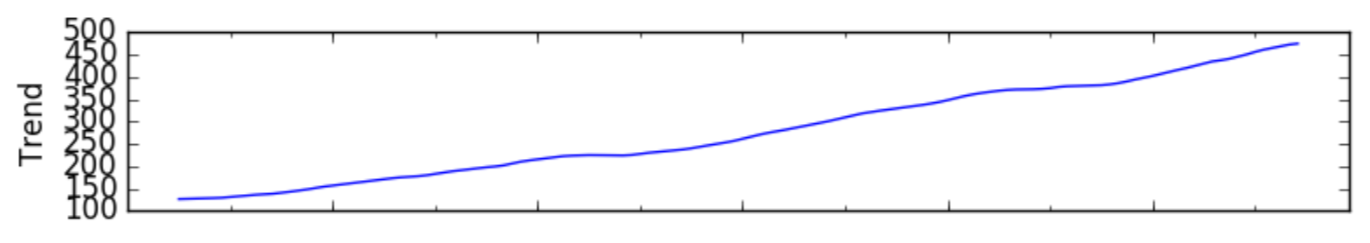
\includegraphics[scale=0.3]{Figures/Trend}
	\decoRule
	\caption[Trend]{Trend \parencite{}}
	\label{fig:Trend}
	%https://medium.com/swlh/time-series-analysis-7006ea1c3326
\end{figure}

\subsubsection{Seasonality}

Seasonality refers to the occurrence of variations on a regular basis. Seasonal variables such as the time of year, day of the week, and other similarities influence the time-series, which is why it is called seasonal. As a result, it has a set period of time that is often limited to a year. A seasonal time-series is depicted in Figure 4 \parencite{Braei2020}.

\begin{figure}[h]
	\centering
	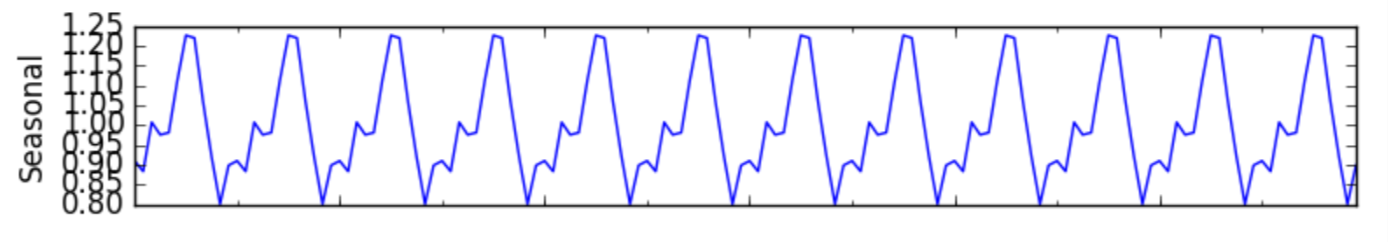
\includegraphics[scale=0.3]{Figures/Seasonal}
	\decoRule
	\caption[Seasonality]{Seasonality \parencite{}}
	\label{fig:Seasonality}
	%https://medium.com/swlh/time-series-analysis-7006ea1c3326
\end{figure}

\subsubsection{Noise}

The variability in the observations that the model cannot account for.

\begin{figure}[h]
	\centering
	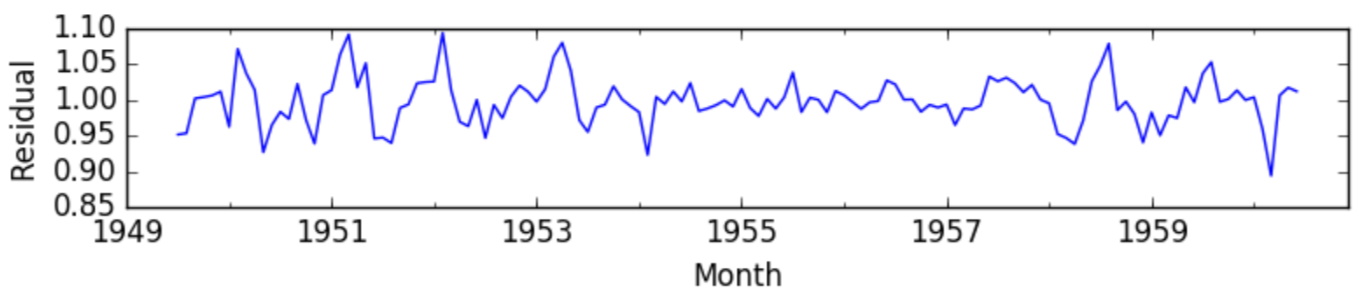
\includegraphics[scale=0.3]{Figures/Residual}
	\decoRule
	\caption[Noise]{Noise \parencite{}}
	\label{fig:Noise}
	%https://medium.com/swlh/time-series-analysis-7006ea1c3326
\end{figure}

\subsubsection{Observed}

All the above componenents combined could provide the observed time series shown in Figure . The components may add up to form a model such as: 

\begin{equation}
	Y =level + trend + seasonality + noise
\end{equation}

\begin{figure}[h]
	\centering
	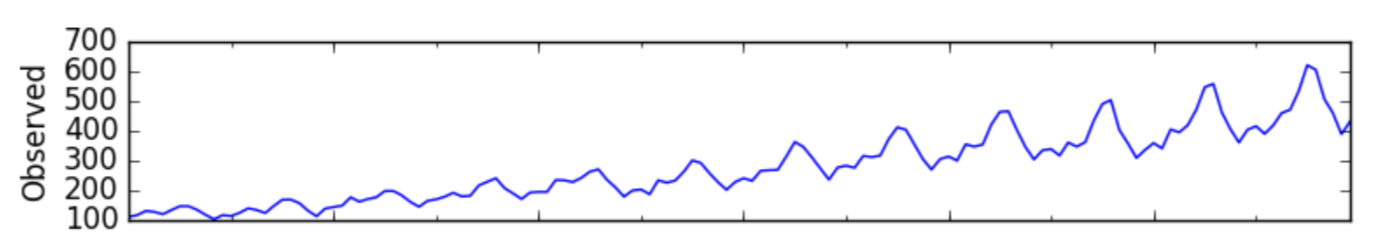
\includegraphics[scale=0.3]{Figures/Observed}
	\decoRule
	\caption[Observed]{Observed \parencite{}}
	\label{fig:Observed}
	%https://medium.com/swlh/time-series-analysis-7006ea1c3326
\end{figure}


\section{RNN for Anomaly Detection}

 -- state of the art

\subsection{CNNs}

\subsection{CNN for time series data}

\subsection{Parameter Settings for fair comparison}

\subsection{Transfer Learning}

\section{Research Gap}
